\documentclass[12pt]{article}
\usepackage{amsmath}
\usepackage{graphicx}
\usepackage{hyperref}
\usepackage{listings}
\usepackage{color}
\usepackage{pythonhighlight}

\title{Operating System Course Report - First Half of the Semester}
\author{A class}
\date{\today}

\begin{document}

\maketitle
\newpage

\tableofcontents
\newpage

\section{Introduction}
This report summarizes the topics covered during the first half of the Operating System course. It includes theoretical concepts, practical implementations, and assignments. The course focuses on the fundamentals of operating systems, including system architecture, process management, CPU scheduling, and deadlock handling.

\section{Course Overview}
\subsection{Objectives}
The main objectives of this course are:
\begin{itemize}
    \item To understand the basic components and architecture of a computer system.
    \item To learn process management, scheduling, and inter-process communication.
    \item To explore file systems, input/output management, and virtualization.
    \item To study the prevention and handling of deadlocks in operating systems.
\end{itemize}

\subsection{Course Structure}
The course is divided into two halves. This report focuses on the first half, which covers:
\begin{itemize}
    \item Basic Concepts and Components of Computer Systems
    \item System Performance and Metrics
    \item System Architecture of Computer Systems
    \item Process Description and Control
    \item Scheduling Algorithms
    \item Process Creation and Termination
    \item Introduction to Threads
    \item File Systems
    \item Input and Output Management
    \item Deadlock Introduction and Prevention
    \item User Interface Management
    \item Virtualization in Operating Systems
\end{itemize}

\section{Topics Covered}

\subsection{Basic Concepts and Components of Computer Systems}
This section explains the fundamental components that make up a computer system, including the CPU, memory, storage, and input/output devices.

\subsection{System Performance and Metrics}
This section introduces various system performance metrics used to measure the efficiency of a computer system, including throughput, response time, and utilization.

\subsection{System Architecture of Computer Systems}
Describes the architecture of modern computer systems, focusing on the interaction between hardware and the operating system.

\subsection{Process Description and Control}
Processes are a central concept in operating systems. This section covers:
\begin{itemize}
    \item Process states and state transitions
    \item Process control block (PCB)
    \item Context switching
\end{itemize}

\subsection{Scheduling Algorithms}
\subsubsection{Round Robbin}
salah satu algoritma penjadwalan proses yang digunakan dalam sistem operasi. Algoritma ini membagi waktu eksekusi secara adil kepada setiap proses yang berjalan dalam sistem dengan prinsip "quantum time". Setelah quantum habis, proses yang sedang berjalan akan ditunda, dan CPU akan diberikan ke proses berikutnya dalam antrian. Algoritma ini berfokus pada fairness atau keadilan dalam pembagian waktu CPU.

\begin{figure}[h]
\centering
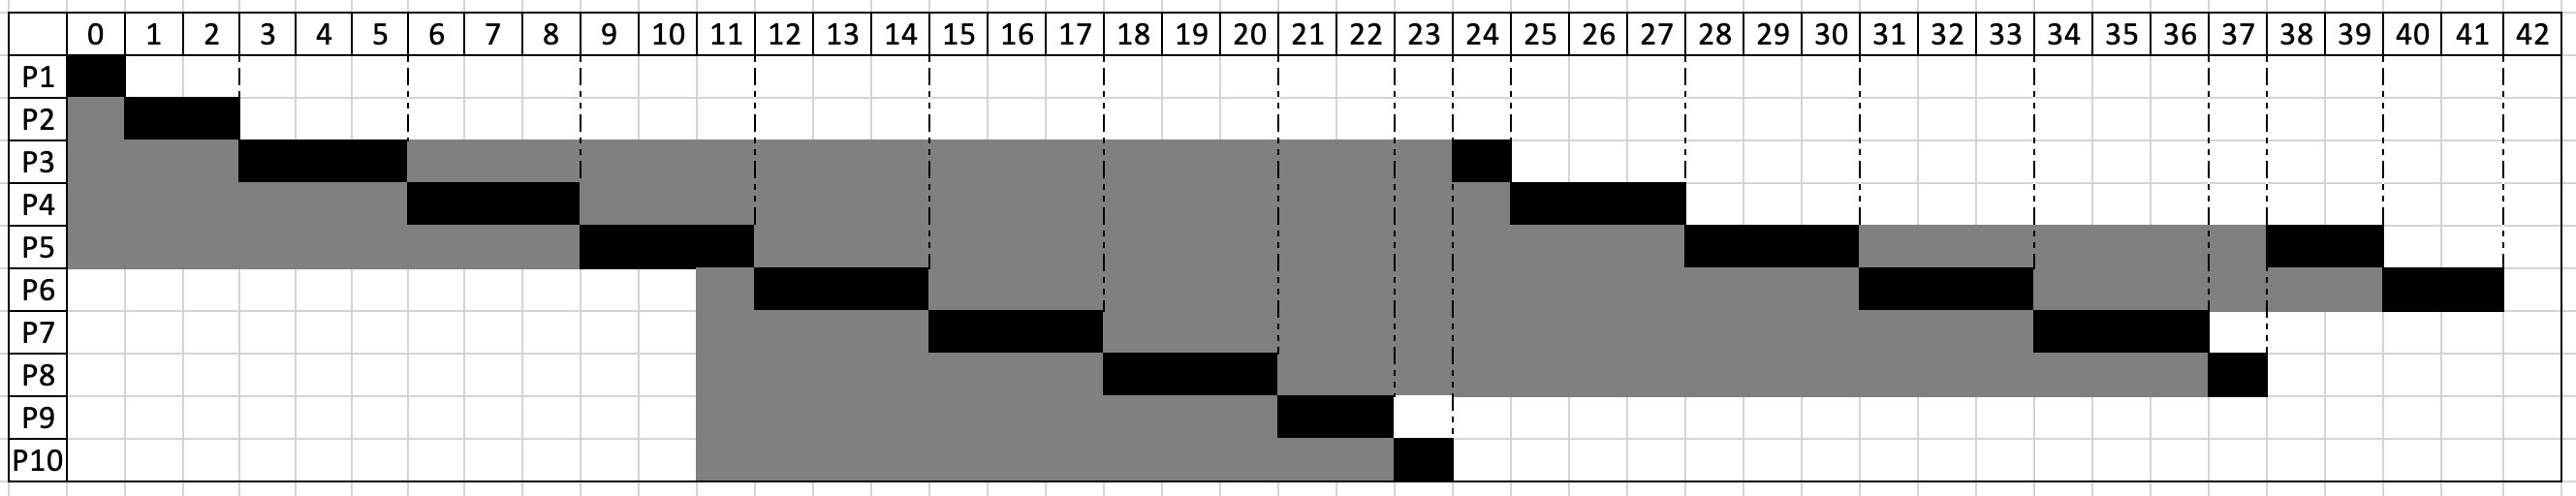
\includegraphics[width=0.6\textwidth]{asset/Kelompok5_Round Robbin.png}
\caption{Ilustrasi Algoritma Round Robin}
\label{fig:roundrobin}
\end{figure}

\begin{itemize}
\item Kelebihan
\begin{itemize}
    \item Setiap proses memiliki kesempatan untuk dieksekusi secara adil dalam waktu yang sama.
    \item Cocok untuk sistem time-sharing.
\end{itemize}
\end{itemize}

\begin{itemize}
\item Kekurangan
\begin{itemize}
    \item Overhead terjadi karena switching antara proses, terutama jika quantum terlalu kecil.
    \item Jika quantum terlalu besar, algoritma ini bisa berubah menjadi FCFS
\end{itemize}
\end{itemize}

\paragraph{Contoh}
 nyata dari algoritma Round Robin dapat dilihat dalam situasi seperti ujian, di mana seorang siswa memiliki sejumlah soal untuk dijawab. Misalnya, setiap soal diberi waktu 2 menit. Jika siswa belum selesai menjawab soal tersebut dalam 2 menit, mereka harus beralih ke soal berikutnya. Setelah semua soal sudah dibaca atau dikerjakan sebentar, siswa kembali ke soal yang belum selesai.
\begin{itemize}
    \item Siswa mulai dengan soal pertama dan memiliki waktu 2 menit untuk menjawab.
    \item Jika belum selesai dalam 2 menit, siswa harus melanjutkan ke soal berikutnya.
    \item Setelah semua soal telah dikerjakan sebentar, siswa kembali ke soal-soal yang belum selesai, dan melanjutkan dari bagian yang tertinggal, lagi-lagi selama 2 menit setiap kali.
    \item Siklus ini berulang sampai semua soal selesai atau waktu ujian habis.
\end{itemize}

\subsection{Process Creation and Termination}
Details how processes are created and terminated by the operating system, including:
\begin{itemize}
    \item Process spawning
    \item Process termination conditions
\end{itemize}

\subsection{Introduction to Threads}
This section introduces the concept of threads and their relation to processes, covering:
\begin{itemize}
    \item Single-threaded vs. multi-threaded processes
    \item Benefits of multithreading
\end{itemize}

\begin{figure}[h]
    \centering
    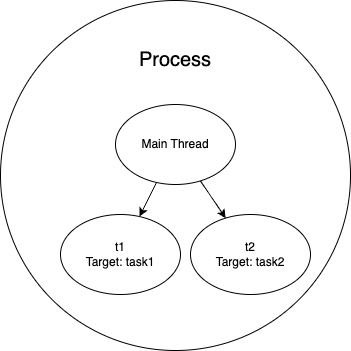
\includegraphics[width=0.5\textwidth]{asset/example.png}  % Sesuaikan nama file dan ukurannya
    \caption{Ini adalah gambar contoh dari multithreading.}
    \label{fig:contoh_gambar}
\end{figure}

Seperti yang terlihat pada Gambar \ref{fig:contoh_gambar}, inilah cara menambahkan gambar dengan keterangan.

\subsection{File Systems}
File systems provide a way for the operating system to store, retrieve, and manage data. This section explains:
\begin{itemize}
    \item File system structure
    \item File access methods
    \item Directory management
\end{itemize}

\subsection{Input and Output Management}
Input and output management is key for handling the interaction between the system and external devices. This section includes:
\begin{itemize}
    \item Device drivers
    \item I/O scheduling
\end{itemize}

\subsection{Deadlock Introduction and Prevention}
Explores the concept of deadlocks and methods for preventing them:
\begin{itemize}
    \item Deadlock conditions
    \item Deadlock prevention techniques
\end{itemize}

\subsection{User Interface Management}
This section discusses the role of the operating system in managing the user interface. Topics covered include:
\begin{itemize}
    \item Graphical User Interface (GUI)
    \item Command-Line Interface (CLI)
    \item Interaction between the user and the operating system
\end{itemize}

\subsection{Virtualization in Operating Systems}
Virtualization allows multiple operating systems to run concurrently on a single physical machine. This section explores:
\begin{itemize}
    \item Concept of virtualization
    \item Hypervisors and their types
    \item Benefits of virtualization in modern computing
\end{itemize}

\section{Assignments and Practical Work}
\subsection{Assignment 1: Process Scheduling}
Students were tasked with implementing various process scheduling algorithms (e.g., FCFS, SJN, and RR) and comparing their performance under different conditions.
\subsubsection{Group 1}
\begin{python}
    class Process:
    def __init__(self, pid, arrival_time, burst_time):
        self.pid = pid
        self.arrival_time = arrival_time
        self.burst_time = burst_time
        self.completion_time = 0
        self.turnaround_time = 0
        self.waiting_time = 0
\end{python}

\begin{table}[htbp] % Optional: For floating position
    \centering
    \begin{tabular}{|c|c|c|} % Defines number of columns and alignment (c = center, l = left, r = right). '|' creates vertical lines.
    \hline
    Header 1 & Header 2 & Header 3 \\ % Column headers
    \hline
    Row 1, Column 1 & Row 1, Column 2 & Row 1, Column 3 \\ % First row of data
    \hline
    Row 2, Column 1 & Row 2, Column 2 & Row 2, Column 3 \\ % Second row of data
    \hline
    \end{tabular}
    \caption{Your table caption} % Optional: For adding a caption
    \label{tab:your_label} % Optional: For cross-referencing the table
\end{table}

\subsubsection{Group 5}
\textbf{Soal:}
Hitung waktu selesai, waktu putar, dan waktu tunggu untuk setiap proses jika menggunakan algoritma FCFS (First Come First Serve), SJN (Shortest Job First), dan RR (Round Robbin).
    \begin{table}[h] % Optional: For floating position
        \centering
        \begin{tabular}{|c|c|c|} % Defines number of columns and alignment (c = center, l = left, r = right). '|' creates vertical lines.
        \hline
        Proses & Waktu Kedatangan & Waktu Burst \\ % Column headers
        \hline
        P1 & 0 & 4 \\ % First row of data
        \hline
        P2 & 1 & 3 \\ % Second row of data
        \hline
        P3 & 2 & 2 \\
        \hline
        P4 & 3 & 1 \\
        \hline
        \end{tabular}
        \caption{Data Proses Untuk Penjadwalan} % Optional: For adding a caption
        \label{tab:Data Proses Untuk Penjadwalan} % Optional: For cross-referencing the table
    \end{table}

    
\begin{python}
Assignment 1 

class Proses:
    def __init__(self, pid, waktu_kedatangan, waktu_burst):
        self.pid = pid  # ID Proses
        self.waktu_kedatangan = waktu_kedatangan  # Waktu kedatangan proses
        self.waktu_burst = waktu_burst  # Waktu eksekusi yang dibutuhkan
        self.waktu_selesai = 0  # Waktu penyelesaian proses
        self.waktu_putar = 0  # Waktu putar (completion - arrival)
        self.waktu_tunggu = 0  # Waktu tunggu (turnaround - burst)

def fcfs(proses_list):
    # Urutkan proses berdasarkan waktu kedatangan
    proses_list.sort(key=lambda x: x.waktu_kedatangan)  
    waktu_sekarang = 0  # Waktu saat ini
    for proses in proses_list:
        # Jika waktu saat ini kurang dari waktu kedatangan, set waktu saat ini ke waktu kedatangan
        if waktu_sekarang < proses.waktu_kedatangan:
            waktu_sekarang = proses.waktu_kedatangan
        waktu_sekarang += proses.waktu_burst  # Tambahkan waktu burst ke waktu saat ini
        proses.waktu_selesai = waktu_sekarang
        proses.waktu_putar = proses.waktu_selesai - proses.waktu_kedatangan
        proses.waktu_tunggu = proses.waktu_putar - proses.waktu_burst

def sjn(proses_list):
    proses_list.sort(key=lambda x: (x.waktu_kedatangan, x.waktu_burst))  # Urutkan berdasarkan arrival dan burst
    waktu_sekarang = 0
    while proses_list:
        # Ambil proses yang sudah tiba
        antrean_siaps = [p for p in proses_list if p.waktu_kedatangan <= waktu_sekarang]
        if not antrean_siaps:
            waktu_sekarang += 1  # Tunggu satu unit waktu
            continue
        # Ambil proses dengan burst time terpendek
        terpendek = min(antrean_siaps, key=lambda x: x.waktu_burst)
        proses_list.remove(terpendek)  # Hapus dari daftar proses
        waktu_sekarang += terpendek.waktu_burst
        terpendek.waktu_selesai = waktu_sekarang
        terpendek.waktu_putar = terpendek.waktu_selesai - terpendek.waktu_kedatangan
        terpendek.waktu_tunggu = terpendek.waktu_putar - terpendek.waktu_burst

def round_robin(proses_list, kuota_waktu):
    antrean = proses_list.copy()  # Salin proses ke antrean
    waktu_sekarang = 0
    while antrean:
        proses = antrean.pop(0)  # Ambil proses dari depan antrean
        if proses.waktu_burst > kuota_waktu:
            waktu_sekarang += kuota_waktu
            proses.waktu_burst -= kuota_waktu  # Kurangi burst time
            antrean.append(proses)  # Masukkan kembali ke antrean
        else:
            waktu_sekarang += proses.waktu_burst
            proses.waktu_selesai = waktu_sekarang
            proses.waktu_putar = proses.waktu_selesai - proses.waktu_kedatangan
            proses.waktu_tunggu = proses.waktu_putar - proses.waktu_burst
            proses.waktu_burst = 0  # Proses telah selesai

\end{python}

\textbf{\textit{Output:}}
\begin{table}[h!]
    \centering
    \begin{tabular}{|c|c|c|c|c|c|}
        \hline
        Proses & Waktu Kedatangan & Waktu Burst & Waktu Selesai & Waktu Putar & Waktu Tunggu \\
        \hline
        P1 & 0 & 4 & 4 & 4 & 0 \\
        \hline
        P2 & 1 & 3 & 7 & 6 & 3 \\
        \hline
        P3 & 2 & 2 & 9 & 7 & 5 \\
        \hline
        P4 & 3 & 1 & 10 & 7 & 6 \\
        \hline
    \end{tabular}
    \caption{Tabel Hasil Algoritma FCFS}
\end{table}

\begin{table}[h!]
    \centering
    \begin{tabular}{|c|c|c|c|c|c|}
        \hline
        Proses & Waktu Kedatangan & Waktu Burst & Waktu Selesai & Waktu Putar & Waktu Tunggu \\
        \hline
        P1 & 0 & 4 & 4 & 4 & 0 \\
        \hline
        P4 & 3 & 1 & 5 & 2 & 1 \\
        \hline
        P3 & 2 & 2 & 7 & 5 & 3 \\
        \hline
        P2 & 1 & 3 & 10 & 9 & 6 \\
        \hline
    \end{tabular}
    \caption{Tabel Hasil Algoritma SJN}
\end{table}

\begin{table}[h!]
    \centering
    \begin{tabular}{|c|c|c|c|c|c|}
        \hline
        Proses & Waktu Kedatangan & Waktu Burst & Waktu Selesai & Waktu Putar & Waktu Tunggu \\
        \hline
        P1 & 0 & 4 & 8 & 8 & 4 \\
        \hline
        P2 & 1 & 3 & 9 & 8 & 5 \\
        \hline
        P3 & 2 & 2 & 7 & 5 & 3 \\
        \hline
        P4 & 3 & 1 & 6 & 3 & 2 \\
        \hline
    \end{tabular}
    \caption{Tabel Hasil Algoritma Round Robin (Quantum = 2)}
\end{table}

\subsection*{Kesimpulan:}
Dari hasil output tersebut, kita bisa menyimpulkan bahwa:

\begin{itemize}
    \item FCFS lebih adil karena memproses sesuai urutan kedatangan, namun dapat menyebabkan waktu tunggu lebih lama untuk proses dengan burst pendek yang datang terlambat.
    \item SJN memberikan waktu tunggu lebih rendah secara keseluruhan, terutama untuk proses dengan burst pendek, tetapi bisa menyebabkan kelaparan (starvation) bagi proses yang datang lebih awal namun memiliki burst besar.
    \item RR memastikan keadilan di antara proses dengan meminimalkan waktu tunggu bagi proses yang seringkali lambat diproses oleh algoritma lain, meski bisa sedikit lebih lama dalam penyelesaian jika quantum-nya kecil.
\end{itemize}

\subsection{Assignment 2: Deadlock Handling}
In this assignment, students were asked to simulate different deadlock scenarios and explore various prevention methods.

\subsection{Assignment 3: Multithreading and Amdahl's Law}
This assignment involved designing a multithreading scenario to solve a computationally intensive problem. Students then applied **Amdahl's Law** to calculate the theoretical speedup of the program as the number of threads increased.

\subsection{Assignment 4: Simple Command-Line Interface (CLI) for User Interface Management}
Students were tasked with creating a simple **CLI** for user interface management. The CLI should support basic commands such as file manipulation (creating, listing, and deleting files), process management, and system status reporting.

\subsection{Assignment 5: File System Access}
In this assignment, students implemented file system access routines, including:
\begin{itemize}
    \item File creation and deletion
    \item Reading from and writing to files
    \item Navigating directories and managing file permissions
\end{itemize}

\section{Conclusion}
The first half of the course introduced core operating system concepts, including process management, scheduling, multithreading, and file system access. These topics provided a foundation for more advanced topics to be covered in the second half of the course.

\end{document}